\documentclass[
  accentcolor=tud1c,	% Color theme for TUD corporate design
  colorbacktitle,		% Titlepage has colored background for title area
  inverttitle,			% Font color of title on titlepage is inverted
  german,
  twoside
]{tudexercise}

\usepackage[ngerman]{babel}
\usepackage{units}
\usepackage{hyperref}
\usepackage{booktabs}
\usepackage[utf8]{inputenc}
\usepackage{algorithm2e}
\usepackage{paralist}

\definecolor{commentgreen}{RGB}{50,127,50}


\usepackage{listings}
\lstloadlanguages{C++,[gnu]make}
\lstset{language=C++}
\lstset{captionpos=b}
\lstset{tabsize=3}
\lstset{breaklines=true}
\lstset{basicstyle=\ttfamily}
\lstset{columns=flexible,keywordstyle=\color{purple},stringstyle=\color{blue},commentstyle=\color{commentgreen}}
\lstset{literate=%
	{Ö}{{\"O}}1
	{Ä}{{\"A}}1
	{Ü}{{\"U}}1
	{ß}{{\ss}}2
	{ü}{{\"u}}1
	{ä}{{\"a}}1
	{ö}{{\"o}}1
	{'}{{\textquotesingle}}1
}

\lstnewenvironment{lstmake} %
{\lstset{language=[gnu]make}} %
{}

\parindent0pt
\parskip2ex


\newcommand{\superscript}[1]{\ensuremath{^{\textrm{#1}}}}
\newcommand{\subscript}[1]{\ensuremath{_{\textrm{#1}}}}

\newcommand{\cppSetTitle}{
	\title{Übung zum\linebreak[1]C/C++-Praktikum\linebreak[1] Fachgebiet Echtzeitsysteme}
	\subtitle{Übungen für den \tag{}. Tag}
}

\newcommand{\cppSetHeaderAndMakeTitle}{
	\begin{examheader}
		\textmb{Übung zum C/C++-Praktikum - Tag \tag{}}
	\end{examheader}
	\maketitle
}

\newcommand{\tag}{1}

\cppSetTitle

\begin{document}

\cppSetHeaderAndMakeTitle 


\section*{Generelle Hinweise}

Die Instruktionen auf den Übungsblättern sind in der Du-Form gehalten; wir hoffen, dass ist kein Problem. :-)

C++ ist nicht einfach zu erlernen; insbesondere die Interpretation der Compilerfehler ist eine Kunst für sich.
\textbf{Bitte aktiv um Hilfe, wenn du nicht weiterkommst.}

\section*{Shortcuts}

Das Arbeiten mit Eclipse macht erst so richtig Spaß, wenn man einige Shortcuts beherrscht.
Dazu zählen:
\begin{description}
	\item[Autocomplete (\emph{Ctrl+Space})]
	Hier erhältst du Vervollständigungsvorschläge und andere Hinweise.
	Versuche es mal mit \emph{std::}, \emph{using namespace}.
	Wenn du \emph{main} tippst und \emph{Ctrl+Space} drückst, generiert Eclipse für dich die \emph{main}-Funktion.
	
	\item[Umbenennen (\emph{Alt+Shift+R})]
	Mit dieser Funktion kannst du Variablen, Funktionen, Klassen,\dots umbenennen.
	
	\item[Neu (\emph{Ctrl+N})]
	Hier kannst du schnell neue Resourcen (Dateien, Projekte,\dots) anlegen.
	
	\item[Header$\leftrightarrow$Source (\emph{Ctrl+Tab})]
	Auf diese Weise kannst du schnell zwischen dem Header und der Implementierungdatei hin- und herspringen.
	
	\item[Go to (\emph{Ctrl+Click}/\emph{F3})] Wenn du \emph{Ctrl} gedrückt hältst und auf ein Element klickst (Funktion, Klasse,\dots), navigiert Eclipse dorthin.
\end{description}

\section*{SVN}

Alle notwendigen Unterlagen wie Übungsblätter, Musterlösungen etc. sind in einem SVN-Repository gesammelt. Es empfiehlt sich diese zu verwenden, denn dort sind die aktuellsten Versionen verfügbar. 

Um den Zugriff über das SVN-Plug-in von Eclipse einzurichten gehst du wie folgt vor:

Über \textbf{\emph{Window $\rightarrow$ Open Perspective $\rightarrow$ SVN Repository Exploring}} öffnet sich eine Ansicht zur Verwaltung deiner Repositories. Es dürften bereits zwei Repositories vorhanden sein - diese kannst du ignorieren. 

Mit einem Rechtsklick im \emph{SVN Repositories}-Tab und dann \textbf{\emph{New $\rightarrow$ Respository Location}} öffnet sich ein Dialog, in dem du eine Adresse für das neue Repository einfügen kannst. Als Adresse gibst du dort folgende Adresse ein:\\[2ex] \emph{https://tud-cpp-praktikum.googlecode.com/svn/trunk/}\\[2ex]
Damit solltest du nun einen neuen Eintrag für das Repository haben.

Mit einem Rechtsklick auf das Repository kannst du \emph{\textbf{Checkout}} auswählen. In dem erscheinenden Dialog kannst du mit einem Klick auf \emph{Finish} das aktuelle SVN-Repository in deinen Workspace kopieren. Im nächsten Dialog suchst du dir einen Namen für das Projekt aus und schließt den Vorgang mit \emph{Finish} ab.

Nun kannst du wieder in den \emph{C/C++}-View wechseln (auch möglich über \textbf{\emph{Window $\rightarrow$ Open Perspective\dots}}). Es sollte ein neues Projekt in deinem Workspace vorhanden sein, das alle Unterlagen enthält.

Neben dem Gesamtprojekt für alle Unterlagen gibt es zum Beispiel für die Musterlösung jeder Aufgabe ein eigenes Unterprojekt.

\section{Eclipse CDT}

Für alle Übungen des C/C++ Praktikums werden wir Eclipse zusammen mit dem C/C++ Development Tooling (CDT) und dem MinGW GCC Compiler verwenden.
Wir gehen davon aus, dass du den generellen Umgang Eclipse bereits aus der Java-Programmierung kennst und nur die Unterschiede zur C++-Programmierung erläutert werden müssen.

Alle Tools sind bereits auf den Poolrechnern vorinstalliert.
Falls du mit deinem Notebook arbeiten möchtest, findest du den Installer (Windows) unter: \url{https://www.dropbox.com/sh/rn714n1ugt6t3ke/AAB2rCt7FCHstSCp_NbnLekya?dl=0}.

Verwende zum Starten von Eclipse den \textbf{\emph{Eclipse für CPPP $\rightarrow$ Eclipse}} Eintrag im Startmenü bzw. das \textbf{\emph{eclipse.cmd}} Script im Installationsordner.
Starte bitte nicht \emph{eclipse.exe} direkt, weil dabei nicht alle benötigten Pfade gesetzt werden.

\subsection{Toolchain einstellen}

Als erstes muss MinGW als die bevorzugte C/C++ Toolchain eingestellt werden.
Öffne dazu den Menüpunkt \textbf{Window $\rightarrow$   Preferences} und wähle \textbf{C/C++ $\rightarrow$  New CDT project wizard}.
Markiere nun \textbf{MinGW GCC} rechts in der Liste und klicke auf \textbf{Make toolchain(s) preferred}.
Schließe den Dialog anschließend mit \textbf{OK}.

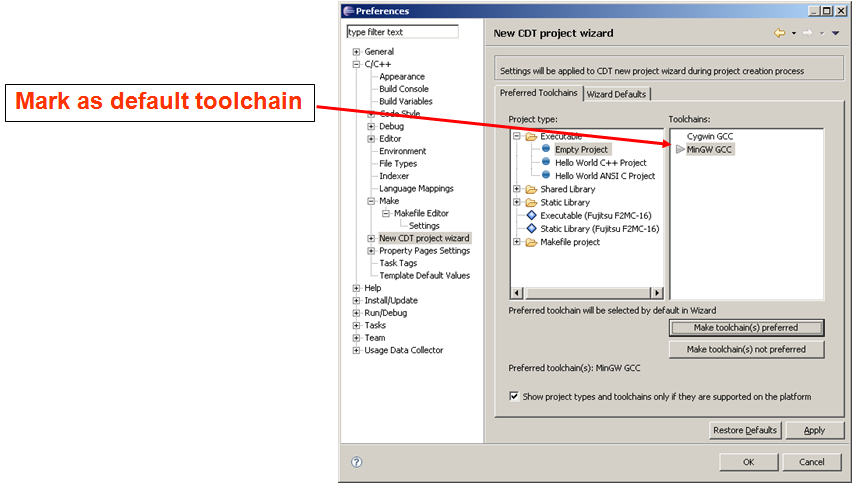
\includegraphics[width=1\textwidth]{toolchain.png}

\subsection{Neues Projekt anlegen}
Um ein neues Projekt anzulegen, wähle \textbf{File $\rightarrow$ New $\rightarrow$ C++ Project} im Eclipse Menü.
Gib den gewünschten Projektnamen ein und wähle \textbf{Empty Project} bzw. \textbf{Hello World C++ Project} als Projekttyp aus.
Die Toolchain sollte bereits automatisch auf MinGW voreingestellt sein.

\begin{center}
	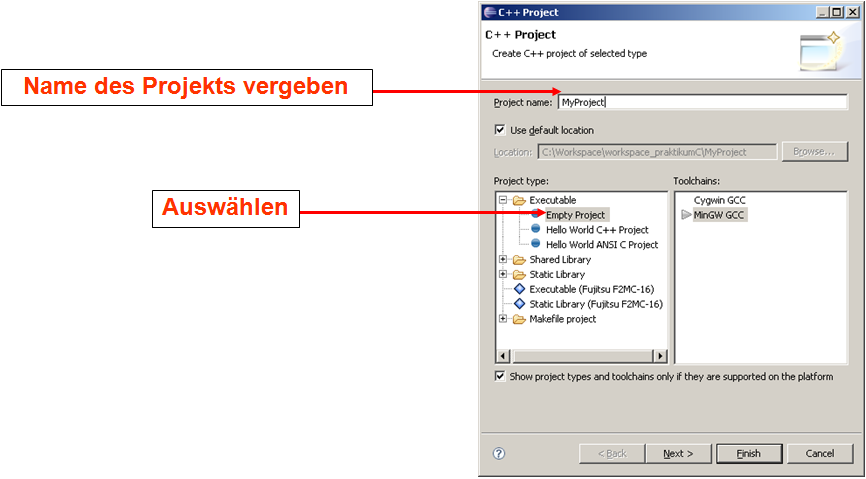
\includegraphics[width=1\textwidth]{new_project.png}
\end{center}

\subsection{Neue Dateien hinzufügen}

Um eine neue Sourcecode-Datei zum Projekt hinzuzufügen, klicke mit der rechten Maustaste auf das Projekt und wähle \textbf{New $\rightarrow$ Source File}.
Gib einen Dateinamen (z.B. \emph{main.cpp}) ein und bestätige mit 
\textbf{Finish}. 
Verfahre analog, um Header-Dateien zu erstellen, wähle jedoch \textbf{New $\rightarrow$ Header File} im Kontextmenü.
Sourcecode-Dateien tragen in der Regel die Endung \emph{.cpp}, Header-Dateien \emph{.h} oder \emph{.hpp} (Wir empfehlen \emph{.h} zu benutzen).

\begin{center}
	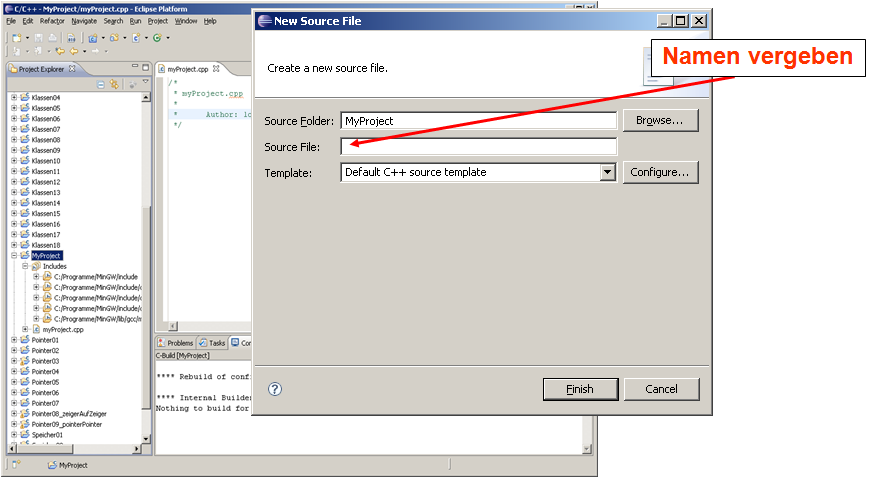
\includegraphics[width=1\textwidth]{new_file.png}
\end{center}

\subsection{Neue Klassen hinzufügen}

Für eine Klasse kann man Header- und Sourcecode-Datei in einem Schritt erzeugen.
Wähle dazu \textbf{New $\rightarrow$ Class} im Kontext-Menü des Projekts, um den entsprechenden Wizard zu starten.
Gib den Namen und bei Bedarf den Namespace sowie weitere Informationen wie z.B. die Elternklassen ein (dazu später mehr).
Setze für die ersten Aufgaben den \textbf{virtual} Modifier des Destruktors auf \textbf{No}.

\begin{center}
	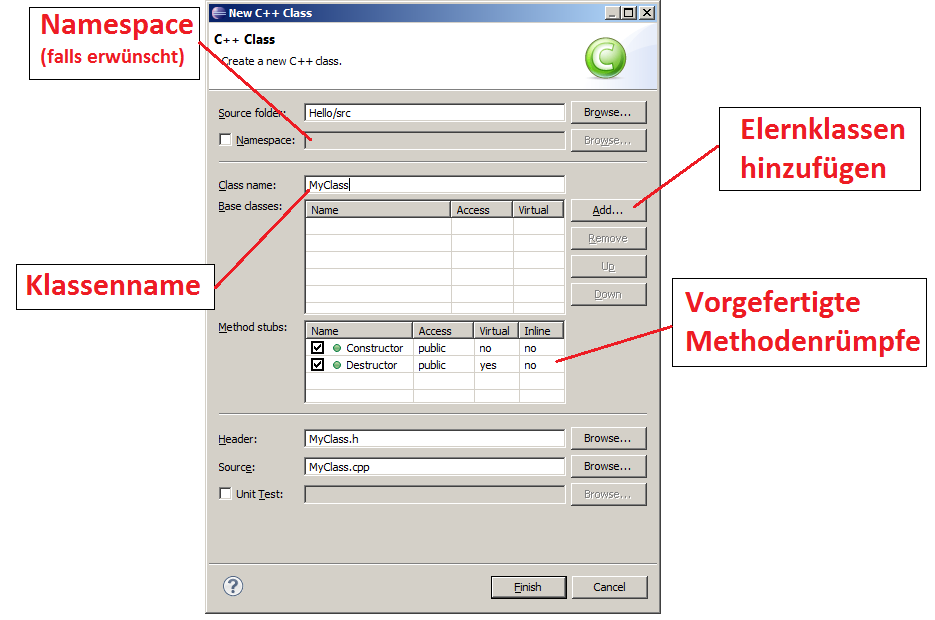
\includegraphics[width=1\textwidth]{class_wizard.png}
\end{center}

\subsection{Projekt kompilieren und starten}

Bevor ein C++-Programm gestartet werden kann, muss es kompiliert werden.
Im Gegensatz zu Java wird der Compiler nicht automatisch von Eclipse im Hintergrund aufgerufen, sondern muss manuell gestartet werden.
Um das aktuell offene Projekt zu kompilieren, klicke auf das \textbf{Build-}Symbol (\glqq Hammer\grqq) in der Eclipse C++ Toolbar.
Im \textbf{Console-}Fenster unten werden Compiler-Meldungen und eventuelle Fehler während des Erstellungsprozesses angezeigt.

Öffne zum Starten des Programms das Kontextmenü des Projekts und wähle \textbf{Run As$\rightarrow$ Local C/C++ Application }.
Danach kannst du zum Starten den grünen Run-Knopf benutzen.

\begin{center}
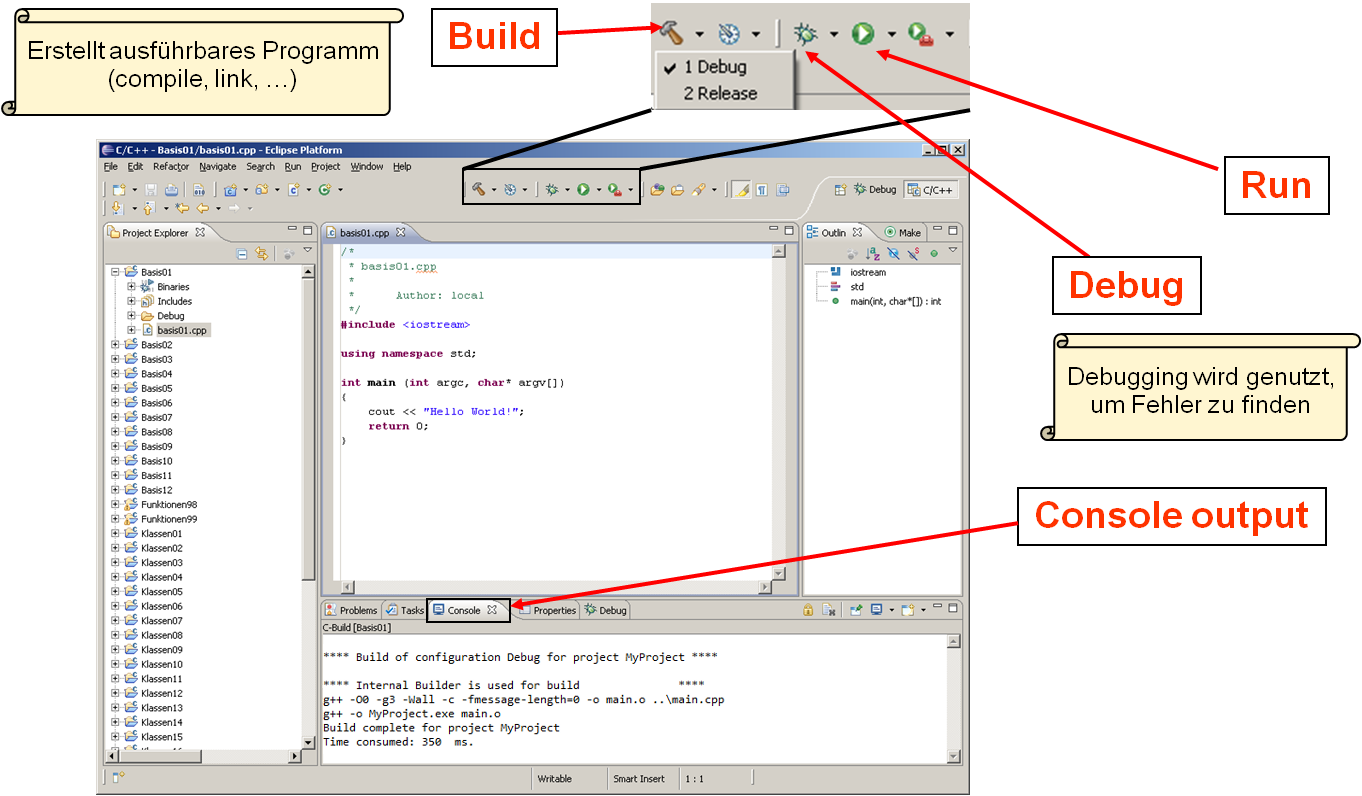
\includegraphics[width=1\textwidth]{build_run.png}
\end{center}

\subsection{Projekt debuggen}
Du kannst dein Programm auch im Debug-Modus laufen lassen, um dir Schritt für Schritt den Ablauf anzusehen und mögliche Fehler zu finden.
Zum Debuggen wählst du (wie auch bei Java) den Debug-Knopf (\glqq Käfer\grqq) und Eclipse wird automatisch in die Debug-Perspektive wechseln.

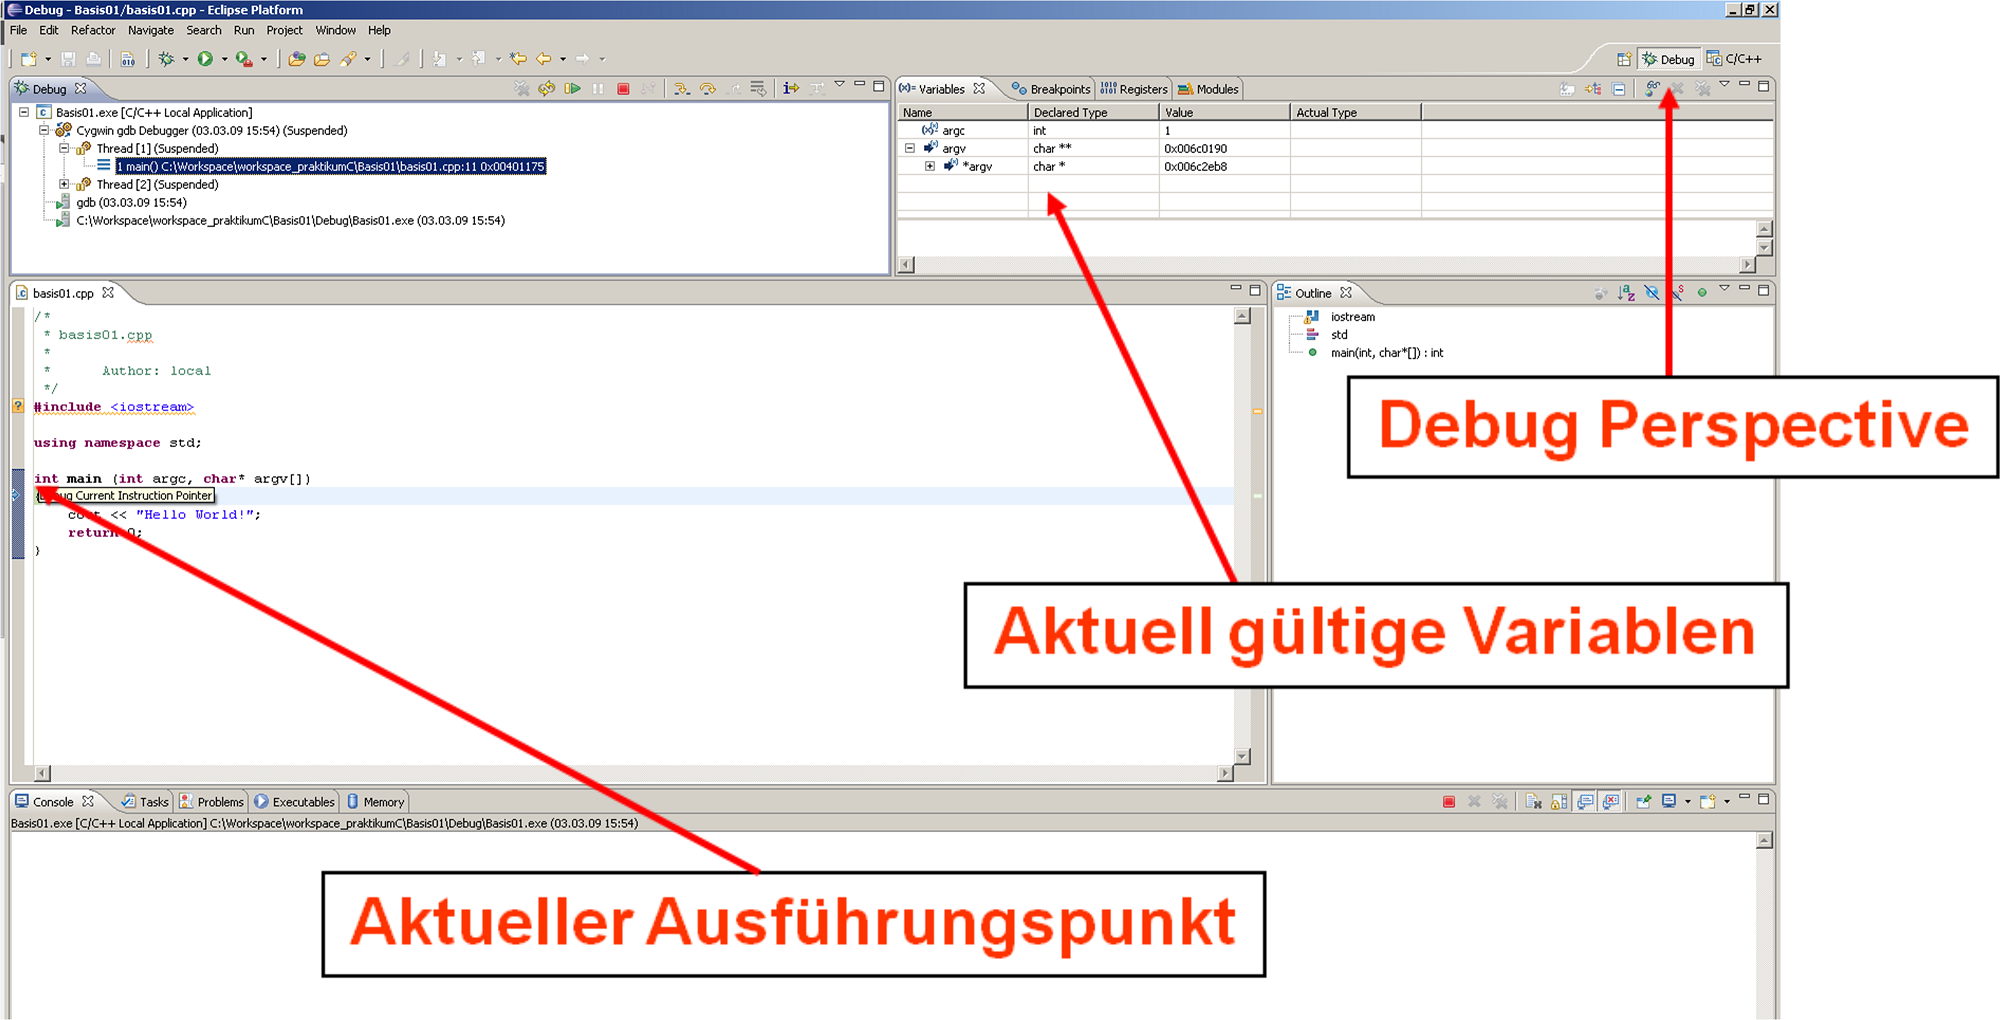
\includegraphics[width=1\textwidth]{debug.png}

\subsection{Erklärung des Hello-World Projekts}
Wenn du \emph{Hello World C++ Project} als Projekttyp auswählst, wird der Wizard automatisch ein Beispiel-Projekt erzeugen, welches \textbf{!!!Hello World!!!} auf der Konsole ausgibt.
Als Einstieg gehen wir im Folgenden den generierten Code durch.

\begin{lstlisting}
	#include <iostream>
\end{lstlisting}

Die erste Zeile bindet den Header \emph{iostream} ein.
Dieser enthält unter anderem Klassen und Funktionen zur Ein- und Ausgabe.
Beachte, dass es zwei verschiedene Möglichkeiten gibt, eine Header-Datei einzubinden -  per \textbf{\#include <...>} sowie per \textbf{\#include "..."}. Bei der ersten Variante sucht der Compiler nur in den Include-Verzeichnissen der Compiler-Toolchain, während bei der zweiten Variante auch die Projektordner durchsucht werden. Somit eignet sich die erste Schreibweise für System-Header und die zweite für eigene, projektspezifische Header.

\begin{lstlisting}
	using namespace std;
\end{lstlisting}
Die zweite Zeile bewirkt, dass der \textbf{Namespace \emph{std} eingebunden} wird. Ähnlich wie Package-Namen in Java dienen Namespaces (Namensräume) in C++ zur Strukturierung des Codes und zur Gruppierung von Elementen wie Funktionen und Klassen.
Durch Namespaces können Namenskonflikte innerhalb von verschiedenen Bibliotheken vermieden werden.
Anders als in Java sind Namespaces in C++ eher kurz, nur sehr selten verschachtelt und nicht an die Ordnerstruktur gebunden.


Der Namespace der C++Standardbibliothek \emph{Standard Template Library (STL)} ist \emph{std}. 
Um ein Element aus der \emph{STL} zu verwenden, müsste man vor jedem Aufruf ein \emph{std::} setzen, z.B. \emph{std::cout} um Ausgaben auf der Konsole zu tätigen.
Indem wir mittels \textbf{using namespace std;} den gesamten Namensraum einbinden, ist dies nicht mehr nötig.
Man kann dies gut mit statischen Imports bei Java vergleichen.
Bei Bedarf können auch einzelne Elemente des Namespaces eingebunden werden, z.B. \textbf{using std::cout;}.

\begin{lstlisting}
	int main() {
		...
	}
\end{lstlisting}

Die \textbf{Main-Funktion} stellt den Einstiegspunkt des Programms dar.
Anders als in Java können Funktionen auch außerhalb von Klassen definiert und verwendet werden.
Der zurückgegebene \emph{int} signalisiert dem Aufrufer (Betriebssystem, Shell,\dots) den Erfolg oder Misserfolg der Ausführung.
Typischerweise bedeutet \textbf{0 Erfolg} und Werte \textbf{kleiner 0 einen Fehler}.

Jedes vollständige C++ Programm muss \textbf{genau eine }\emph{main()}-Funktion besitzen. Andernfalls wird der Linker mit der Fehlermeldung \emph{undefined reference to 'main'} abbrechen.

\begin{lstlisting}
	cout << "!!!Hello World!!!" << endl; // prints !!!Hello World!!!
\end{lstlisting}
Durch \textbf{cout $<<$ ... $<<$ ...} können Werte auf der Konsole ausgegeben werden\footnote{
Für weitere Informationen zur Kommandozeilenausgabe siehe \url{http://www.cplusplus.com/doc/tutorial/basic_io/} und \url{http://www.cplusplus.com/reference/iomanip/}.
}.
Ein \textbf{endl} beendet die aktuelle Zeile mit einem Zeilenvorschub.
\textbf{//} leitet einen einzeiligen Kommentar ein.
Mehrzeilige Kommentare werden in \textbf{/* ... */} eingeschlossen.

\subsection{Häufige Compiler-Fehlermeldungen des gcc}

\begin{verbatim}
error: expected ';' before ...
\end{verbatim}

Dies bedeutet, dass in der Zeile davor ein \textbf{;} vergessen wurde.
Allgemein beziehen sich Fehlermeldungen \textbf{expected ... before ...} häufig auf die Zeile \textbf{vor} dem markierten Statement.
Beachte, dass \emph{die Zeile davor} auch die letzte Zeile einer eingebundenen Header-Datei sein kann. Beispiel:

\begin{lstlisting}
#include "main.h"
int main() {
	...
}
\end{lstlisting}

Falls im Header \emph{main.h} in der letzten Zeile ein Semikolon fehlt, wird der Compiler die Fehlermeldung trotzdem auf die Zeile \textbf{int main() \{} beziehen!!

\begin{verbatim}
error: invalid conversion from <A> to <B>.
\end{verbatim}

Dies bedeutet, dass der Compiler an der entsprechenden Stelle einen Ausdruck vom Typ \emph{B} erwartet, im Code jedoch ein Ausdruck vom Typ \emph{A} angegeben wurde. Insbesondere bei verschachtelten Typen sowie (später vorgestellten) Zeigern und Templates kann die Fehlermeldung sehr lang werden. In so einem Fall lohnt es sich, den Ausdruck in mehrere Teilausdrücke aufzubrechen und die Teilergebnisse durch temporäre Variablen weiterzureichen.

\begin{verbatim}
undefined reference to ...
\end{verbatim}

Dies bedeutet, dass das Programm zwar korrekt kompiliert wurde, der Linker aber die Definition des entsprechenden Bezeichners nicht finden kann.
Das kann passieren, wenn man dem Compiler durch einen Prototypen mitteilt, dass eine bestimmte Funktion existiert (\textbf{deklariert}), diese aber nirgendwo tatsächlich \textbf{definiert}.
Überprüfe in diesem Fall, ob der Bezeichner tatsächlich definiert wurde und ob die Signatur der Definition mit dem Prototypen übereinstimmt.


\subsection{Primitive Datentypen}
Die primitiven Datentypen in C++ sind ähnlich denen in Java.
Allerdings sind alle Ganzzahl-Typen in C++ sowohl mit als auch ohne Vorzeichen verfügbar.
Standardmäßig sind Zahlen vorzeichenbehaftet.
Mittels \textbf{unsigned} kann man vorzeichenlose Variablen deklarieren.
Durch das freie Vorzeichenbit kann ein größerer positiver Wertebereich dargestellt werden.

\begin{lstlisting}
 	int i; // signed int, -2147483648 to +2147483647 on 32-bit machine
	unsigned int ui; // unsigned int, 0 to 4294967295 on 32-bit machine
	// unsigned double d; // not possible
\end{lstlisting}

Eine andere Besonderheit von C++ ist, dass Ganzzahlwerte implizit in Boolesche Werte (Typ: \emph{bool}) umgewandelt werden.
Alles ungleich 0 wird als \textbf{true} gewertet, 0 als \textbf{false}.
Somit können Ganzzahlen direkt in Bedingungen ausgewertet werden:

\begin{lstlisting}
 	int n = 5;
 	// loop which runs until n is 0
 	while(n--) { // post-decrement n, i.e. decrement n but return previous value
  		cout << n << endl;
 	}

	// output: 4 3 2 1 0
\end{lstlisting}


\section{C++ Grundlagen, Funktionen und Strukturierung}

Nach dieser kurzen Einführung darfst du dir jetzt selber die Hände schmutzig machen.

Wir lernen als zunächst die Kontrollstrukturen (if/for/while) von C++ kennen, die weitgehend gleich sind wie in Java.
In den folgenden Aufgaben werden die Unterschiede und Gemeinsamkeiten stückweise erläutert.

\begin{enumerate}

\item Lege ein neues \glqq{}Hello World\grqq{}-Projekt an (\emph{File} $\rightarrow$ \emph{New} $\rightarrow$ \emph{C++ Project} $\rightarrow$ \emph{Hello World C++ Project}).
Kompiliere und starte das Programm.

Jetzt haben wir einen Ausgangspunkt für eine eigene Implementierung.


\item 
Schreibe eine Funktion \emph{printStars(int n)}\footnote{Was die Benennung von Funktionen, Variablen und Klassen angeht, bist du frei.
Für Klassen ist CamelCase wie in Java üblich. Bei Funktionen und Variablen wird zumeist entweder auch Camel Case oder Kleinschreibung mit Unterstrichen verwendet.}, die \emph{n}-mal ein \textbf{*} auf der Konsole ausgibt und mit einem Zeilenvorschub abschließt.
Ein Aufruf von \emph{printStars(5)} sollte folgende Ausgabe generieren:
\begin{lstlisting}
*****
\end{lstlisting}

Platziere die Funktion \emph{vor} der \emph{main}, da sie sonst von dort aus nicht aufgerufen werden kann.
Benutze die erstellte Funktion \emph{printStars(int n)}, um eine weitere Funktion zu schreiben, die eine Figur wie unten dargestellt ausgibt.
Verwende hierzu Schleifen.
\begin{lstlisting}
*****
****
***
**
*
**
***
****
*****
\end{lstlisting}

\item
Lagere dein Programm aus Aufgabenteil b) in eine eigene Datei aus.
Gehe dazu folgendermaßen vor: 

Erstelle eine neue Header-Datei \emph{functions.h} und eine neue Sourcecode-Datei \emph{functions.cpp}. 

Binde \emph{functions.h} in beide Sourcecode-Dateien mittels 
einer \textbf{\#include} ein.
Vergiss nicht, auch in \emph{functions.cpp} den \emph{std}-Namespace sowie \emph{iostream} einzubinden, falls du dort Elemente der Standardbibliothek benutzen möchtest.

Vermeide bei größeren Programmen bitte unbedingt, den Namespace bereits im Header einzubinden!
Dadurch würden alle Dateien, die den Header einbinden, den Namespace ebenfalls einbinden, was zu Namenskonflikten und anderen hässlichen Überraschungen führen kann.
Benutze daher im Header immer voll qualifizierte Bezeichner (z.B. \emph{std::string}, \emph{std::ostream}).

Schreibe nun in \emph{functions.h} \textbf{Funktionsprototypen} für die beiden Funktionen aus b).
Funktionsprototypen dienen dazu, dem Compiler mitzuteilen, dass eine Funktion mit bestimmtem Namen, Parametern und Rückgabewert existiert.
Ein Prototyp ist im wesentlichen eine mit \textbf{;} abgeschlossene Signatur der Funktion ohne Funktionsrumpf.
Der Prototyp von \emph{printStars(int n)} lautet \emph{void printStars(int n);}

Verschiebe deine beiden Funktionen nach \emph{functions.cpp}.
Fertig -- die Ausgabe des Programms sollte sich nicht verändert haben.

\item
Erweitere das in Aufgabenteil c) erstellte Programm um eine Eingabeaufforderung zur Bestimmung der Breite der auszugebenden Figur.
Die Breite soll dabei eine im Programmcode vorgegebene Grenze nicht überschreiten dürfen.
Gib gegebenenfalls eine Fehlermeldung aus.
Zum Einlesen verwendest du \texttt{cin >{}> \emph{variable}}.
Erstelle auch für diesen Aufgabenteil eine eigene Funktion und lagere diese nach \emph{functions.cpp} aus.

\item Statt eines einzelnen Zeichens soll nun das fortlaufende Alphabet ausgegeben werden.
Sobald das Ende des Alphabets erreicht wurde, beginnt die Ausgabe erneut bei \emph{a}. Beispiel:
\begin{lstlisting}
abc
de
f
gh
ijk
\end{lstlisting}

Implementiere dazu eine Funktion \emph{char nextChar()}.
Diese soll bei jedem Aufruf das nächste auszugebende Zeichen von Typ \emph{char} zurückgeben, beginnend bei \emph{\textquotesingle a\textquotesingle}.
Dazu muss sich \emph{nextChar()} intern das aktuelle Zeichen merken.
Dies kann durch die Verwendung von \emph{static}-Variablen erreicht werden. \emph{static}-Variablen sind Variablen, die ihren alten Wert beim Wiedereintritt in die Funktion annehmen.
Ein statische Variable \emph{c} wird mittels 
\begin{lstlisting}
static char c = 'a';
\end{lstlisting}
deklariert.
In diesem Fall wird c \textbf{einmalig zu Beginn des Programms} mit 'a' initialisiert und kann später beliebig verändert werden.
\end{enumerate} 

\section{Klassen}

In der vorherigen Übung haben wir den Modifier \textbf{static} verwendet, um eine Funktion zu erstellen, welche fortlaufende Zeichen generiert.
Diese Methode hat jedoch mehrere Nachteile, unter anderem kann man die Funktion nicht in mehreren Threads gleichzeitig nutzen.
Deshalb werden wir nun eine Klasse schreiben, die das aktuelle Zeichen als Attribut enthält und durch Methoden ausgelesen und inkrementiert werden kann.

\begin{enumerate}

\item
Lege ein neues Projekt an und füge dem Projekt eine neue leere Klasse \emph{CharGenerator} hinzu.
Obwohl Eclipse Klassenrümpfe automatisch generieren kann, wollen wir aus Übungsgründen die Klasse diesmal manuell erstellen.
Erzeuge dazu einen Header \emph{CharGenerator.h} und eine Sourcecode-Datei \emph{CharGenerator.cpp}.
Binde \emph{CharGenerator.h} in \emph{CharGenerator.cpp} und in \emph{main.cpp} ein.

Erstelle nun den Klassenrumpf von \emph{CharGenerator} in der Header-Datei. Die allgemeine Syntax lautet hierbei 

\begin{lstlisting}
class MyClass {  
}; // semi-colon!
\end{lstlisting}

Genauso wie bei Funktionen wird auch bei Methoden von Klassen zwischen Deklaration und Implementierung unterschieden.
Die Struktur der Klasse mit allen Attributen und Methodenprototypen wird im Header beschrieben, während die Sourcecode-Datei nur Implementierungen enthält.
Da wir noch keine Methoden definiert haben, ist unsere Sourcecode-Datei entsprechend leer.

\item
Füge Ihrer Klasse nun das \emph{private} Attribut \emph{char nextChar} hinzu, in dem das als nächstes auszugebende Zeichen gespeichert wird. Im Gegensatz zu Java  werden in C++ die Access-Modifier \emph{public}/\emph{private}/\emph{protected} nicht bei jeder Methode einzeln sondern blockweise angegeben. Dazu wird der jeweilige Access-Modifier an die gewünschte Stelle in der Klassendeklaration geschrieben und mit einem Doppelpunkt abgeschlossen.  Alle darauffolgenden Deklarationen werden nun unter diesem Modifier erstellt. Beispiel:

\begin{lstlisting}
class Foo { 
public:
	void iAmPublic(); // public method
	// more public members
protected:
	void iAmProtected(); // protected method
	// more protected members
private:
	void iAmPrivate(); // private method
	...
};
\end{lstlisting}

Füge das Attribut \emph{nextChar} als \textbf{private} hinzu.

\item
Noch wurde \emph{nextChar} kein Wert zugewiesen.
Das wollen wir nun nachholen und einen Konstruktor für die Klasse \emph{CharGenerator} erstellen, der \emph{nextChar} auf einen Anfangswert setzt.
Der Konstruktor wird als eine Methode ohne Rückgabetyp deklariert, die den gleichen Namen wie die Klasse hat, und beliebige Parameter beinhalten kann, in unserem Fall zunächst 
\begin{lstlisting}
CharGenerator();
\end{lstlisting}

Erstelle den Konstruktorprototypen im \emph{public}-Bereich der Klasse und eine Implementierung in der Sourcecode-Datei. Damit der Compiler weiß, zu welcher Klasse eine Methode/Konstruktor gehört, muss man vor dem Methodennamen den Scope der Klasse angeben.

\begin{lstlisting}
CharGenerator::CharGenerator() {  // Konstruktor von CharGenerator.
	...
}
\end{lstlisting}

Um \emph{nextChar} einen Wert zuzuweisen, werden wir eine sogenannte Initialisierungsliste verwenden.
Diese beschreibt, wie die Attribute einer Klasse initialisiert werden.
Dadurch wird garantiert, dass beim Eintritt in den Konstruktorrumpf alle Objektattribute bereits initialisiert sind und verwendet werden dürfen.

Die Initialisierungsliste wird durch einen Doppelpunkt zwischen der schließenden Klammer der Parameterliste und der geschweiften Klammer des Rumpfes eingeleitet, und bildet eine mit Komma separierte Liste von Attributennamen und ihren Initialisierungsargumenten in Klammern.

Die Reihenfolge der Initialisierungsliste sollte der Deklarationsreihenfolge entsprechen.
Konstanten \emph{müssen} in der Initialisierungsliste zugewiesen werden.

Beispiel:

\begin{lstlisting}
CharGenerator::CharGenerator(): nextChar('a') {
}
\end{lstlisting}

Initialisiere nun \emph{nextChar} mit 'a' wie beschrieben.

\item
Schreibe nun eine \emph{public} Methode \emph{char generateNextChar()} die analog zur vorherigen Aufgabe das nächste auszugebende Zeichen zurückgibt.
Teile die Methode in Prototyp und Implementierung auf.
Vergiss auch hier nicht, den Scope der Klasse bei der Implementierung anzugeben:

\begin{lstlisting}
char CharGenerator::generateNextChar() {
	...
}
\end{lstlisting}

\item
Teste deine Implementierung.
Lege in der \emph{main}-Funktion ein \emph{CharGenerator}-Objekt mittels \textbf{CharGenerator charGen;} an.
Ein \textbf{new} ist dabei nicht erforderlich (näheres dazu in der nächsten Vorlesung).

Rufe \emph{generateNextChar()} einige Male auf und überprüfe das Ergebnis über die Konsole oder den Debugger.

\item
Wir wollen nun angeben können, mit welchem Zeichen unser \emph{CharGenerator} beginnen soll.
Erweitere dazu den Konstruktor um einen Parameter \emph{char initialChar} und ändere die Initialisierung von \emph{nextChar}, damit dieser mit dem übergebenen Parameter gestartet wird.

Damit man nicht immer das Startzeichen angeben muss, kann man sogenannte \emph{Default Parameter} angeben.
Weise hierzu den Parameter im Prototypen einfach einen Wert zu.
An der Implementierung muss nichts geändert werden.
\begin{lstlisting}
class CharGenerator {
public:
	CharGenerator(char initialChar = 'a');
	...
};
\end{lstlisting}

Nun ist die Angabe des Startzeichens optional und kann auf Wunsch weggelassen werden.
Bei der Definition eines Default-Parameters müssen für alle nachfolgenden Parameter ebenfalls Default-Werte angegeben werden, um Mehrdeutigkeiten beim Aufruf zu vermeiden. 

Teste deine Implementierung sowohl mit als auch ohne Angabe des Startzeichens.
Um ein Startzeichen anzugeben, lege das Objekt wie folgt an:
\begin{lstlisting}
CharGenerator charGen('x');
\end{lstlisting}


\item
Erstelle eine neue Klasse \emph{PatternPrinter} und füge ein \emph{CharGenerator}-Objekt \emph{charGenerator} als privates Attribut hinzu.
Erstelle auch einen leeren, parameterlosen Konstruktor für \emph{PatternPrinter}.

Ohne eine Initialisierungsliste wird \emph{charGenerator} mit dem Default-Parameter initialisiert.
Um ein eigenes Startzeichen anzugeben, muss eine Initialisierungsliste erstellt und \emph{charGenerator} mit dem entsprechenden Argument initialisiert werden.

\item
Erstelle die Methoden \emph{void printNChars(int n)}, \emph{int readWidth()} und \emph{void printPattern()}, die entsprechend \emph{n} Zeichen auf die Konsole ausgeben, die Breite einlesen und unter Verwendungen aller Methoden das Muster aus der vorherigen Aufgabe auf der Konsole ausgeben.
\emph{printNChars} sollte hierbei \emph{charGenerator} benutzen, um das nächste Zeichen ermitteln.

Teste deine Implementierung, indem du ein \emph{PatternPrinter}-Objekt anlegst und \emph{printPattern()} darauf aufrufst.

\end{enumerate}

\section{Operatorüberladung} 
In C++ besteht die Möglichkeit, Operatoren wie \textbf{+} (\emph{operator+}), \textbf{*} (\emph{operator*}),\dots zu überladen.
Man kann selber spezifizieren, was beim Verknüpfen von Objekten mit einem Operator geschehen soll, um zum Beispiel den Quellcode übersichtlicher zu gestalten.
Du hast bereits das Objekt \emph{cout} der Klasse \emph{ostream} kennengelernt, welche den $<<$-Operator überlädt, um Ausgaben von \emph{std::string}, \emph{int},\dots komfortabel zu tätigen.
In dieser Aufgabe wollen wir eine eigene Vektor-Klasse schreiben und einige Operatoren überladen.

Wir werden am Tag 4 auf dieser Aufgabe aufbauen und den Vektor um weitere Funktionen erweitern.
Wirf deine Lösung also bitte nicht direkt weg.
Falls du mit dieser Aufgabe bis dahin nicht fertig sein solltest, kannst du natürlich auf die Musterlösung zurückgreifen.

\begin{enumerate}
\item \textbf{Konstruktor}
Schreibe eine Klasse \emph{Vector3} mit den Attributen \emph{a}, \emph{b} und \emph{c} vom Typ \emph{double}, die die einzelnen Komponenten eines 3-dimensionalen Vektors darstellen.
Die Klasse soll drei Konstruktoren besitzen, einen parameterlosen \textbf{Default-Konstruktor}, der den Vektor mit \textbf{0} initialisiert, einen \textbf{Konstruktor mit 3 Parametern}, der die einzelnen Vektor-Komponenten auf die gegebenen Werte setzt, und einen \textbf{Copy-Konstruktor}.

Der Copy-Konstruktor wird aufgerufen, wenn das Objekt kopiert werden soll, z.B. für eine Call-by-Value Parameterübergabe.
Er nimmt ein Objekt vom gleichen Typ wie die Klasse selbst (in unserem Fall \emph{Vector3}) als Parameter und kopiert alle Attribute.
Die Übergabe sollte dabei per const Reference geschehen.
Näheres dazu in der Vorlesung\footnote{Erklärung: Würden wir \emph{other} by-Value übergeben, müsste eine Kopie von \emph{other} angelegt werden.
	Dazu würde der Copy-Konstruktor aufgerufen, was zu einer unendlichen Rekursion führt, bis der Stack seine maximale Größe überschreitet und das Programm abstürzt.}.
Bis dahin übernimm einfach die folgende Syntax für den Prototypen:
\begin{lstlisting}
Vector3(const Vector3& other);
\end{lstlisting} 

Dadurch kannst du \emph{other} wie ein gewöhnliches \emph{Vector3}-Objekt verwenden, es jedoch nicht verändern.

Füge jedem Konstruktor eine Ausgabe auf der Konsole hinzu, um beim Programmlauf den Lebenszyklus der Objekte nachvollziehen zu können

\item \textbf{Destruktor}

Erstelle außerdem einen Destruktor.
Ein Destruktor ist eine Methode, die automatisch beim Löschen des Objektes aufgerufen wird. Die Syntax des Prototypen lautet
\begin{lstlisting}
~Vector3();
\end{lstlisting} 

und die Implementierung entsprechend
\begin{lstlisting}
Vector3::~Vector3() {
	...
}
\end{lstlisting} 

Füge dem Destruktor eine Ausgabe auf der Konsole hinzu, um beim Programmlauf den Lebenszyklus der Objekte nachvollziehen zu können

\item\textbf{Vektoraddition}
Überlade den Operator \textbf{+} der Klasse \emph{Vector3}, der eine komponentenweise Vektoraddition durchführt.
Die Signatur lautet
\begin{lstlisting}
Vector3 operator+(Vector3 rhs);
\end{lstlisting}
Das \emph{Vector3} links ist dabei der Rückgabetyp der Überladung, der Parameter rhs die rechte Seite (\glqq right-hand-side\grqq{}) des \textbf{+}-Operators.
Dadurch, dass du den Operator als Member der Klasse deklarierst, nimmt die aktuelle Instanz hierbei automatisch die linke Seite der Operation an.
Platziere den Prototyp im \emph{public}-Bereich der \emph{Vector3} Klasse.

Die Implementierung lautet dementsprechend:
\begin{lstlisting}
Vector3 Vector3::operator+(Vector3 rhs) {
	...
}
\end{lstlisting}

Du kannst nun innerhalb der Methode durch \emph{a}, \emph{b} und \emph{c} auf eigene Attribute und über  \emph{rhs.a}, \emph{rhs.b} und \emph{rhs.c} auf Attribute der rechten Seite zugreifen.

\item\textbf{Vektorsubtraktion und Skalarprodukt}\\[0ex]
Überlade auf die gleiche Weise auch die Operatoren $-$ für eine komponentenweise Vektorsubtraktion sowie \textbf{*} für ein Skalarprodukt.
Der Rückgabetyp eines Skalarprodukts ist kein \emph{Vector3} sondern ein Skalar (\emph{double})!

Jetzt kannst du Vektoren durch \emph{v1 + v2}, \emph{v1 - v2} und \emph{v1 * v2} addieren/subtrahieren und das Skalarprodukt bilden.

\item\textbf{Ausgabeoperator (\emph{\texttt{operator<<}})}
Um die Korrektheit unserer Implementierung zu testen, brauchen wie eine Ausgabemöglichkeit eines \emph{Vektor3}-Objektes, idealerweise mit der gewohnten \emph{cout \textbf{$<<$} ...} Syntax.
Dazu überladen wir den \textbf{$<<$} Operator.

Diesmal müssen wir die Überladung \textbf{außerhalb} der \emph{Vektor3}-Klasse definieren, weil auf unser \emph{Vektor3}-Objekt nun auf der rechten Seite der Operation steht. Der Funktionsprototyp lautet 
\begin{lstlisting}
std::ostream& operator<<(std::ostream& out, Vector3 rhs);
\end{lstlisting}

Als linke Seite wird hierbei ein \emph{ostream}-Objekt (wie z.B. \emph{cout}) erwartet.
Um Ausgabeketten \emph{cout} \textbf{$<<$} \dots \textbf{$<<$} \dots zu ermöglichen, muss das Ausgabeobjekt auch zurückgegeben werden. Damit das \emph{ostream}-Objekt nicht jedes Mal kopiert wird, wird es als Referenz \textbf{\&} durchgereicht.

Die Implementierung hat folgende Form:
\begin{lstlisting}
ostream& operator<<(ostream& out, Vector3 rhs)  {
	out << ... ;
	return out;
}
\end{lstlisting}

Fülle die Funktion aus und kompiliere das Projekt.
Vergiss nicht, den \emph{iostream} Header und \emph{std} Namespace einzubinden.

\item\textbf{Komponenten-Getter}
Der Compiler wird mit der Fehlermeldung 
\begin{verbatim}
error: 'double Vector3::a' is private within this context
\end{verbatim}
abbrechen.
Dies liegt daran, dass die Attribute \emph{a}, \emph{b} und \emph{c} privat und nur innerhalb der Klasse sichtbar sind.
Erstelle deshalb Getter-Methoden für die einzelnen Vektorkomponenten und verwende diese in der Ausgabefunktion.
Wenn alles funktioniert hat, kannst du beliebige \emph{Vector3}-Objekte ausgeben:
\begin{lstlisting}
cout << v << endl;
\end{lstlisting} 

\item\textbf{Testen}
Teste deine bisher definierten Methoden und Funktionen.
Probiere auch Kombinationen von verschiedenen Operatoren aus und beobachte das Ergebnis.
Schreibe auch eine einfache Funktion, die Vektoren als Parameter nimmt. 
Wie du siehst, werden sehr viele \emph{Vector3}-Objekte erstellt, kopiert und gelöscht.
Dies liegt daran, dass die Objekte immer per Call-By-Value übergeben und dabei kopiert werden.
Wie dies vermieden werden kann, sehen wir im nächsten Teil des Praktikums.

\end{enumerate}


\section{Aufzug}
In dieser Aufgabe soll ein Grundgerüst für den in der Vorlesung vorgestellten Aufzug-Simulator geschaffen werden.
Folgendes Klassendiagramm veranschaulicht die Klassenstruktur.

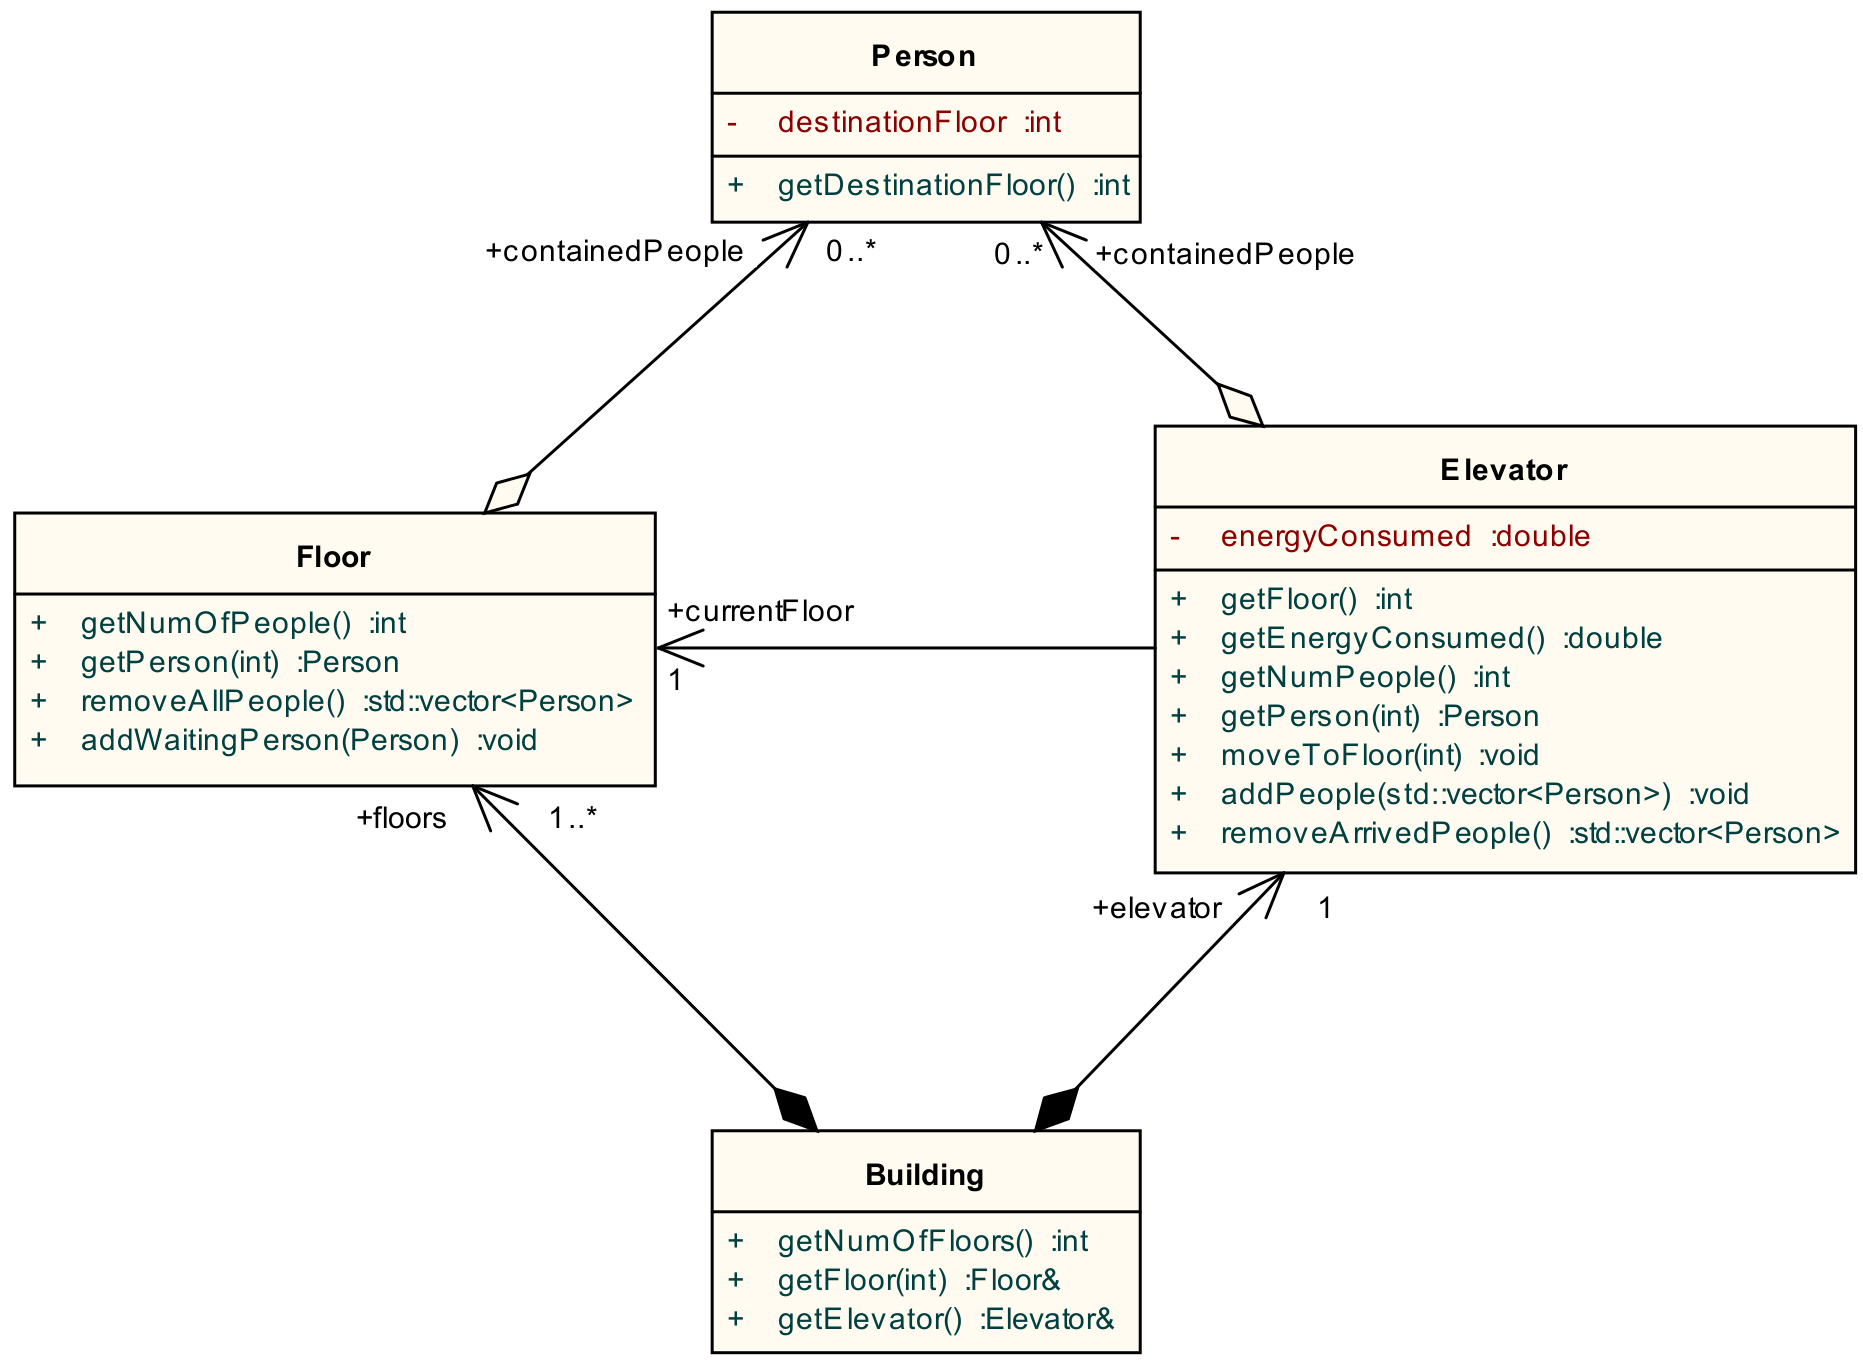
\includegraphics{Aufzug.png}

\begin{enumerate}
\item \textbf{Klasse Person}
Schreibe eine Klasse \emph{Person}.
Diese soll ein Attribut \emph{int destinationFloor} haben, welches das Zielstockwerk angibt. 
Initialisiere das Attribut im Konstruktor und schreibe einen entsprechenden Getter.
Füge dem Konstruktor außerdem eine Ausgabe auf die Konsole hinzu, um später beim Programmlauf den Erzeugungsprozess besser nachvollziehen zu können.
Erstelle zudem einen Destruktor für \emph{Person} sowie den Copy-Konstruktor.
Vergiss nicht, im Copy-Konstruktor \emph{destinationFloor} des anderes Objekts zu übernehmen.
Erstelle auch hier eine Konsolenausgabe, um den Lebenszyklus darzustellen.

\item \textbf{Klasse Elevator}
Schreibe eine Klasse \emph{Elevator} mit den Attributen \emph{int currentFloor}, \emph{double energyConsumed} sowie \emph{std::vector<Person> containedPeople}.
Dabei soll \emph{int currentFloor} die Nummer des aktuellen Stockwerks repräsentieren, \emph{double energyConsumed} die verbrauchte Energie. 
In \emph{containedPeople} werden die sich aktuell im Aufzug befindlichen Menschen gespeichert.
Dafür benutzen wir die Klasse \emph{vector} aus dem \emph{std} Namespace.
Binde dazu den Header \emph{vector} ein.
Der Container \emph{vector} kapselt ein Array und stellt eine ähnliche Funktionalität wie Javas \emph{Vector} Klasse bereit.
Der Typ in spitzen Klammern (\emph{<Person>} in \emph{std::vector<Person>}) ist ein Template-Parameter und besagt, dass in dem Container \emph{Person}-Objekte gespeichert werden sollen.

Schreibe Getter für \emph{currentFloor} und \emph{energyConsumed}.
Implementiere außerdem die Methoden
\begin{lstlisting}
	/** Returns number of people in Elevator */
	int getNumPeople();
	
	/** Returns i-th Person in Elevator */
	Person getPerson(int i);
\end{lstlisting} 

Du kannst mit \emph{containedPeople.size()} auf die Länge eines \emph{vector}s zugreifen und mittels \emph{containedPeople.at(i)} auf das i-te Element. \\

Implementiere auch die Methode
\begin{lstlisting}
	/** Moves the elevator to given floor */
	void moveToFloor(int floor);
\end{lstlisting}

die den Aufzug zu einem bestimmten Stockwerk bewegt.
Passe die verbrauchte Energie sinnvoll an; addiere beispielsweise die Differenz zwischen dem aktuellen und dem Zielstockwerk hinzu.

Als letztes müssen wir die Methoden zum Ein- und Aussteigen implementieren:
\begin{lstlisting}
	/** Adds people to Elevator */
	void addPeople(std::vector<Person> people);

	/** Removes people which arrived at their destination */
	std::vector<Person> removeArrivedPeople();
\end{lstlisting} 

Du kannst dabei \emph{containedPeople.push\_back(Person)} nutzen, um eine einzelne Person zur Menge der Insassen hinzuzufügen. 
Um die Leute aussteigen zu lassen, die an ihrem Zielstockwerk angekommen sind, erstelle in der Methode zwei temporäre \emph{vector}-Container   \emph{stay} und \emph{arrived}. 
Iteriere nun über alle Leute im Aufzug und prüfe, ob das Zielstockwerk der Person mit dem aktuellen Stockwerk des Aufzugs übereinstimmt.
Wenn ja, lasse die Person aussteigen, indem du sie zu der \emph{arrived}-Liste mittels \emph{push\_back()} hinzufügst.
Andernfalls muss die Person im Aufzug verbleiben (\emph{stay}-Liste). 
Gib am Ende die arrived-Liste zurück, und ersetze \emph{containedPeople} durch \emph{stay}.

\item \textbf{Klasse Floor}
Schreibe die Klasse \emph{Floor} mit dem Attribut \emph{std::vector<Person> containedPeople}.
Implementiere die folgenden Methoden:

\begin{lstlisting}
	/** Returns number of people on this floor */
	int getNumPeople();
	
	/** Returns i-th Person on this floor */
	Person getPerson(int i);
	
	/** Adds a Person to this floor */
	void addWaitingPerson(Person h);
	
	/** Removes all persons from this floor and return them */
	std::vector<Person> removeAllPeople();
\end{lstlisting}

Nutze \emph{containedPeople.clear()} um alle Elemente eines \emph{vector}s zu löschen.

\item\textbf{Klasse Building}
Schreibe eine Klasse \emph{Building}.
Der Konstruktor soll dabei die Anzahl der Stockwerke als Parameter erhalten.
Füge einen Aufzug \emph{elevator} sowie \emph{std::vector<Floor> floors} als private Attribute hinzu.
Implementiere einen Getter, der den Aufzug als Referenz (\emph{Elevator\&}) zurückgibt.
Implementiere dazu die folgenden Methoden:

\begin{lstlisting}
	/** Returns number of floors */
	int getNumOfFloors();
	
	/** Returns a certain floor as reference*/
	Floor& getFloor(int floor);
\end{lstlisting}


\item 
Um die Benutzung des Simulators von außen zu vereinfachen und lange Aufrufketten wie
\begin{lstlisting}
	b.getElevator().addPeople(b.getFloor(b.getElevator().getFloor()).removeAllPeople());
\end{lstlisting} 

zu vermeiden, werden wir \emph{Building} einige weitere Methoden hinzufügen.
Der Simulator sollte nur mit Methoden der Klasse \emph{Building} kommunizieren.
Implementiere hierfür folgende Komfortmethoden:

\begin{lstlisting}
	/** 
	 * Lets people on current floor go into the elevator.
	 */
	void letPeopleIn();
	
	/** Removes people from elevator on current floor which arrived at their destination */
	std::vector<Person> removeArrivedPeople();
	
	/** Moves the building's elevator to given floor */
	void moveElevatorToFloor(int i);
	
	/** Adds a person to given floor */
	void addWaitingPerson(int floor, Person p);
\end{lstlisting}	

\item
Teste deine Implementierung.
Erstelle dazu zunächst ein Gebäude und füge einige Personen hinzu.

\begin{lstlisting}
	Building b(3);
	b.addWaitingPerson(0, Person(2)); // person in floor 0 wants to floor 2
	b.addWaitingPerson(1, Person(0)); // person in floor 1 wants to floor 0
	b.addWaitingPerson(2, Person(0)); // person in floor 2 wants to floor 0
\end{lstlisting}

Implementiere nun folgende Beförderungsstrategie.
Diese sehr einfache (und ineffiziente) Strategie fährt alle Stockwerke nacheinander ab, sammelt die Leute ein und befördert sie jeweils zu ihren Zielstockwerken.

\begin{algorithm}[H]
 \SetAlgoLined
 \For{Floor floor \textbf{in} Building}{
   Move \emph{elevator} to Floor \emph{floor};\\
   Let all people on \emph{floor} into \emph{elevator};\\
   
  \While{elevator has people} {
    Move Elevator to destination Floor of first Person in Elevator; \\
    Remove arrived people; \\
  }
 }
\end{algorithm}

Gib am Ende auch die verbrauchte Energie aus.
Schau dir die Ausgabe genau an und versuche nachzuvollziehen, warum Personen so oft kopiert werden.
Denke daran, dass diese bei einer Übergabe als Argument kopiert werden.
\end{enumerate}

\end{document}
